%The KamLAND-Zen experiment will search for \bbonu\ in \XE\ using enriched xenon dissolved in liquid scintillator. This will allow a calorimetric measurement of the \bb\ electrons, as first proposed in \cite{Raghavan:1994qw}. Xenon is relatively easy to dissolve (with a mass fraction of more than 3\% being possible) and also easy to extract from the scintillator. 

%The major modification to the existing KamLAND detector \cite{KamLAND:2002uet} was the construction of an inner, very radiopure (of order $3\times 10^{-12}$ g/g of \URANIUM\ and \THORIUM) and very transparent balloon to hold the dissolved xenon. This balloon, 1.58 m in radius, is placed at the center of the KamLAND active volume as shown in fig.~\ref{fig:kamlandzen}.

%%%%%
%\begin{figure}[t!]
%\begin{center}
%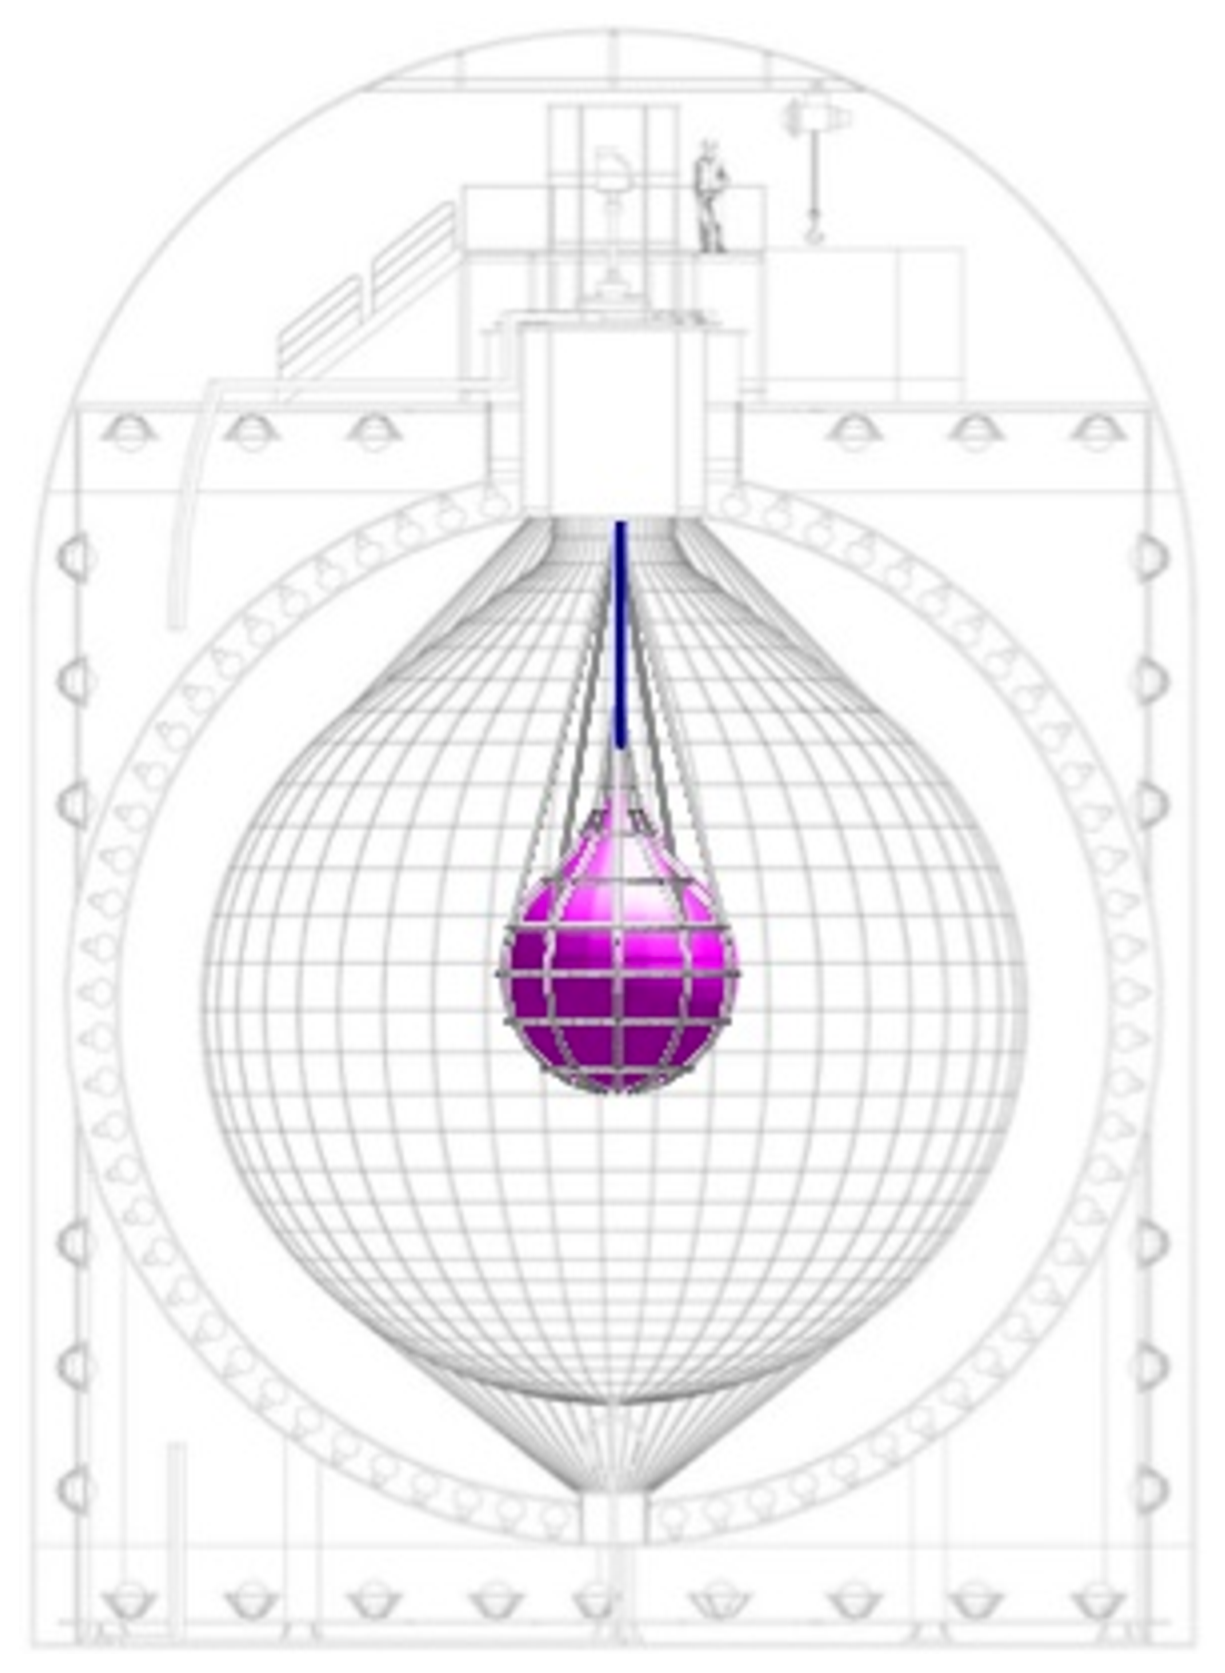
\includegraphics[scale=0.25]{img/kamlandzen.eps}
%\end{center}
%\caption{Sketch of the KamLAND-Zen detector. The ball-on containing the dissolved xenon (purple) hangs in the center of the active volume.} %\label{fig:kamlandzen}
%\end{figure}
%%%%%%

%The KamLAND-Zen experiment plans to dissolve 389 kg of \XE\ in the liquid scintillator of KamLAND in the first phase of the experiment, and up to 1 ton in a projected second phase. 

%The proven resolution (from the previous operation of the KamLAND experiment) is 16\% FWHM at 1 MeV. The main sources of expected background are the \bbtnu\ tail, \BI\ impurities in the scintillator or in the balloon, $^{10}$C generated in the scintillator by cosmic rays, and $^{8}$B solar neutrinos. The expected background rate in the region of interest is $2\times10^{-4}$ \ckky\ \cite{kozlov2011status}, corresponding to $2.2\times10^{-4}$ \ckkbby .

%At the time of writing this report, the mini-balloon installation into the KamLAND detector has been completed, and detector commissioning is ongoing. Physics data-taking with the xenon-loaded liquid scintillator is expected to start in the fall of 2011.



%--------------------------------------------


The KamLAND-Zen experiment is a neutrinoless double beta decay search conducted using the KamLAND detector, a liquid scintillator-based neutrino detector located in the Kamioka mine in Japan. The experiment utilises a large volume of liquid scintillator, doped with a high concentration of Xenon enriched in the Xe136 isotope to enhance the sensitivity to neutrinoless double beta decay.

The KamLAND-Zen detector re-uses the KamLand facility, a spherical volume filled with approximately 1000 tons of liquid scintillator. This volume, designed originally to detect MeV neutrinos, have a very low concentration of $^{238}$U and $^{232}$Th, at the level of 5.0x10$^{-18}$ and 1.3x10$^{-17}$ respectively and it is used in Kamland-Zen as active veto. At the center of this volume, a smaller balloon made out of ethylene-vinylalcohol co-polymer and nylon with a 6.5 m radius and 135 $\mu$m thickness defines a different scintillating volume with xenon dissolve in it. This design allows for accumulation of large amounts of isotope in a very clean environment, the detector configuration also allows to reconstruct the position of the events, allowing to select events far from the ballon walls.
On the other hand as the measurement is based only on the scintillation light, they lack of a good energy resolution producing relatively large background rates in their region of interest when compared with other experiments. In addition, the capabilities of KamLAND-Zen to distinguish among different type of particle interactions is very reduce, although some efforts using neural networks \cite{https://arxiv.org/abs/2203.01870} allow for slightly improved background rejection.
Another issue they face due to their large volume is the relevant contribution to the total background of spallation products that forces to add analysis cuts to select event separated enough in time from muon-induced showers.


%%%%%
\begin{figure}[t!]
\begin{center}
\includegraphics[scale=0.25]{img/KL_fidutial}
\includegraphics[scale=0.25]{img/KL_LD_events}
\end{center}
\caption{Top:Vertex distribution of candidate events (black points) overlaid on $^{214}$Bi background events from the MC simulation (color histogram) in the energy region 2.35 < E < 2.70 MeV (\bbonu\ window), with arbitrary normalization. The solid and thick dashed lines indicate the shape of the IB and the 1.57-m-radius spherical volume, respectively. The dot-dashed line indicates the nylon belt suspending the inner ballon. The thin dashed lines illustrate the shape of the equal-volume spherical half-shells, which compose the 2.5-m-radius spherical fiducial volume. The high-count region at the IB bottom indicates the hot spot and is vetoed.
Bottom:Energy spectra of selected ββ candidates within a 1.57-m-radius spherical volume drawn together with best-fit backgrounds, the 2νββ decay spectrum, and the 90\% C.L. upper limit for \bbonu\ decay of  long-lived data (LD).
} \label{fig:kamlandzen}
\end{figure}
%%%%%%


The current phase of the KamLAND-Zen experiment uses 745 kg of xenon enriched at the 91\% level in the \XE\ isotope \cite{https://arxiv.org/abs/2203.02139}. This is nearly a factor of two in active mass with respect the previous phase of the experiment. The KL collaboration has recently published the results of their last period of data taking \cite{https://arxiv.org/abs/2203.02139} that corresponds to a total exposure of 970 kg yr of \XE\ . Along this period they observe a total of 24 background events, which can be described by the background-dominated approximation. In this analysis they do not find event excess over the expected background setting a limit to the  half-limit in Xe that corresponds to $T_{1/2} > 2.0X10^{26}$ yr (90\% C.L.), even when their sensitivity was 1.3X10$^{26}$. The combined analysis of this data with the KamLAND-Zen 400 pushes further this limit to $T_{1/2} > 2.3X10^{26}$ yr (90\% C.L.), being the best world limit to this process for xenon.
These results set upper limits on the effective Majorana mass of 36-156 meV depending of the NMEs used.
